%iffalse
\let\negmedspace\undefined
\let\negthickspace\undefined
\documentclass[journal,12pt,onecolumn]{IEEEtran}
\usepackage[version=4]{mhchem}
\usepackage{chemformula} % for \ch if needed
\usepackage{chemfig}
\usepackage{chemmacros}
\chemsetup{modules = reactions} % Enables reaction arrows
\usepackage{graphicx}
\graphicspath{ {./images/} }
\usepackage{geometry}
\usepackage{lastpage}
\usepackage{cite}
\usepackage{amsmath,amssymb,amsfonts,amsthm}
\usepackage{enumitem,multicol}
\usepackage{algorithmic}
\usepackage{graphicx}
\usepackage{textcomp}
\usepackage{xcolor}
\usepackage{txfonts}
\usepackage{listings}
\usepackage{enumitem}
\usepackage{mathtools}
\usepackage{gensymb}
\usepackage{comment}
\usepackage[breaklinks=true]{hyperref}
\usepackage{tkz-euclide} 
\usepackage{listings}
\usepackage{gvv}                                        
%\def\inputGnumericTable{}                                 
\usepackage[latin1]{inputenc}                                
\usepackage{color}                                            
\usepackage{array}                                            
\usepackage{longtable}                                       
\usepackage{calc}                                             
\usepackage{multirow}                                         
\usepackage{hhline}                                           
\usepackage{ifthen}                                           
\usepackage{lscape}
\usepackage{tabularx}
\usepackage{array}
\usepackage{float}


\newtheorem{theorem}{Theorem}[section]
\newtheorem{problem}{Problem}
\newtheorem{proposition}{Proposition}[section]
\newtheorem{lemma}{Lemma}[section]
\newtheorem{corollary}[theorem]{Corollary}
\newtheorem{example}{Example}[section]
\newtheorem{definition}[problem]{Definition}
\newcommand{\BEQA}{\begin{eqnarray}}
\newcommand{\EEQA}{\end{eqnarray}}
\newcommand{\define}{\stackrel{\triangle}{=}}
\theoremstyle{remark}

\geometry{margin=1 in}



\setlength{\headheight}{14pt}
\setlength{\headsep}{5pt}
\setlength{\footskip}{20pt}

\begin{document}

\begin{enumerate}
   \subsection*{1 to 25 carry one mark each}

\item If matrix 
\[
A = \begin{bmatrix} 2 & 4 \\ 1 & 3 \end{bmatrix}, \quad 
B = \begin{bmatrix} 4 & 6 \\ 5 & 9 \end{bmatrix},
\]
the transpose of product of these two matrices, i.e. $(AB)^T$ is equal to

\begin{multicols}{2}
\begin{enumerate}
    \item $\begin{bmatrix} 28 & 19 \\ 34 & 47 \end{bmatrix}$
    \item $\begin{bmatrix} 19 & 34 \\ 47 & 28 \end{bmatrix}$
    \item $\begin{bmatrix} 48 & 33 \\ 28 & 19 \end{bmatrix}$
    \item $\begin{bmatrix} 28 & 19 \\ 48 & 33 \end{bmatrix}$
\end{enumerate}
\end{multicols}
\hfill{GATE 2011 PI}

\item If $A(0,4,3)$, $B(0,0,0)$ and $C(3,0,4)$ are three points defined in $x,y,z$ coordinate system, then which one of the following vectors is perpendicular to both the line vectors $\overrightarrow{BA}$ and $\overrightarrow{BC}$?

\begin{multicols}{2}
\begin{enumerate}
    \item $16\hat{i} + 9\hat{j} - 12\hat{k}$
    \item $16\hat{i} - 9\hat{j} + 12\hat{k}$
    \item $16\hat{i} - 9\hat{j} - 12\hat{k}$
    \item $16\hat{i} + 9\hat{j} + 12\hat{k}$
\end{enumerate}
\end{multicols}
\hfill{GATE 2011 PI}

\item The solution of the differential equation 
\[
\frac{d^2y}{dx^2} + 6 \frac{dy}{dx} + 9y = 9x + 6
\]
with $C_1$ and $C_2$ as constants is

\begin{multicols}{2}
\begin{enumerate}
    \item $y = (C_1 x + C_2)e^{-3x}$
    \item $y = C_1 e^{3x} + C_2 e^{-3x} + x$
    \item $y = (C_1 x + C_2)e^{-3x} + x$
    \item $y = (C_1 x + C_2)e^{3x} + x$
\end{enumerate}
\end{multicols}
\hfill{GATE 2011 PI}
\item The line integral 
\[
\int_{P_1}^{P_2} \left( y \, dx + x \, dy \right)
\]
from $P_1(x_1, y_1)$ to $P_2(x_2, y_2)$ along the semi-circle $P_1 P_2$ shown in the figure is
\begin{figure}[H]
    \centering
    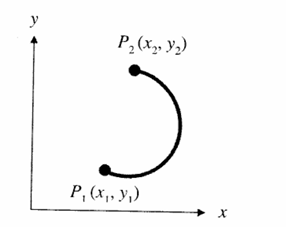
\includegraphics[width=0.25\linewidth]{figs/Q.4.png}
    \caption{fig1}
    \label{fig:figs/Q.4.png}
\end{figure}
\hfill{GATE 2011 PI}
\begin{enumerate}
\begin{multicols}{2}
    \item $x_2y_2 - x_1y_1$
    \item $(y_2^2 - y_1^2) + (x_2^2 - x_1^2)$
    \item $(x_2 - x_1)(y_2 - y_1)$
    \item $(y_2 - y_1)^2 + (x_2 - x_1)^2$
\end{multicols}
\end{enumerate}
\item It is estimated that the average number of events during a year is three. What is the probability of occurrence of not more than two events over a two-year duration? Assume that the number of events follows a Poisson distribution.  

\hfill GATE 2011 PI  

\begin{enumerate}
\begin{multicols}{2}
    \item 0.052
    \item 0.062
    \item 0.072
    \item 0.082
\end{multicols}
\end{enumerate}

\item 
A cirular steel shaft is under elastic deformation due to torsion. The relationship between modulus of elasticity(E) and shear modulus of elasticity(G). taking V as poison's ratio, is 
\hfill GATE 2011 PI  

\begin{enumerate}
\begin{multicols}{2}
    \item $G = 2E(1+\nu)$
    \item $E = 2G(1+\nu)$
    \item $G = \dfrac{2E}{(1+\nu)}$
    \item $E = \dfrac{2G}{(1+\nu)}$
\end{multicols}
\end{enumerate}
\item 
Two circular steel bars having same length L are subjected to equal load P. The first bar has diameter d over its entire length while the second has diameter 2d over two-thirds of its length  as shown in the figure. Assuming linear elastic behaviour, the ratio of strain energy of the first bar to that of second bar is

\begin{figure}[H]
    \centering
    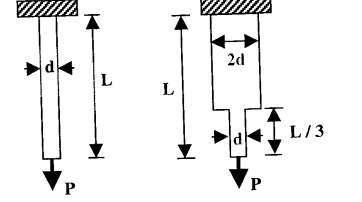
\includegraphics[width=0.5\linewidth]{figs/Q.7.png}
    \caption{fig2}
    \label{fig:figs/Q.7.png}
\end{figure}
\hfill{GATE 2011 PI}
\begin{enumerate}
\begin{multicols}{4}
    \item 1/2
    \item 4
    \item 1/4
    \item 2
\end{multicols}
 \end{enumerate}
 \item An ideal air standard Diesel cycle does NOT contain the following process:  

\hfill GATE 2011 PI  

\begin{enumerate}
\begin{multicols}{2}
    \item constant volume heat addition
    \item constant volume heat rejection
    \item isentropic compression
    \item isentropic expansion
\end{multicols}
\end{enumerate}

\item Which of the following is a surface (two-dimensional) imperfection in the crystal structure of common metals?  

\hfill GATE 2011 PI  

\begin{enumerate}
\begin{multicols}{2}
    \item Vacancy
    \item Dislocation
    \item Grain boundary
    \item Inclusion
\end{multicols}
\end{enumerate}

\item In sand casting, fluidity of the molten metal increases with  

\hfill GATE 2011 PI  

\begin{enumerate}
\begin{multicols}{2}
    \item increase in degree of superheat
    \item decrease in pouring rate
    \item increase in thermal conductivity of the mould
    \item increase in sand grain size
\end{multicols}
\end{enumerate}

\item Which of the following casting processes uses expendable pattern and expendable mould?  

\hfill GATE 2011 PI  

\begin{enumerate}
\begin{multicols}{2}
    \item Shell mould casting
    \item Investment casting
    \item Pressure die casting
    \item Centrifugal casting
\end{multicols}
\end{enumerate}

\item Which of the following welding processes results in the smallest heat affected zone?  

\hfill GATE 2011 PI  

\begin{enumerate}
\begin{multicols}{2}
    \item Shielded metal arc welding
    \item Gas welding
    \item Laser beam welding
    \item Thermit welding
\end{multicols}
\end{enumerate}

\item In resistance seam welding, the electrode is in the form of a  

\hfill GATE 2011 PI  

\begin{enumerate}
\begin{multicols}{2}
    \item cylinder
    \item flat plate
    \item coil of wire
    \item circular disc
\end{multicols}
\end{enumerate}

\item Which of the following powder production methods produces spongy and porous particles?  

\hfill GATE 2011 PI  

\begin{enumerate}
\begin{multicols}{2}
    \item Atomization
    \item Reduction of metal oxides
    \item Electrolytic deposition
    \item Pulverization
\end{multicols}
\end{enumerate}

\item The binding material used in cemented carbide cutting tools is  

\hfill GATE 2011 PI  

\begin{enumerate}
\begin{multicols}{2}
    \item graphite
    \item tungsten
    \item nickel
    \item cobalt
\end{multicols}
\end{enumerate}
\item Grinding ratio is defined as  

\hfill GATE 2011 PI  

\begin{enumerate}
\begin{multicols}{2}
    \item $\dfrac{\text{volume of wheel wear}}{\text{volume of work material removed}}$
    \item $\dfrac{\text{volume of work material removed}}{\text{volume of wheel wear}}$
    \item $\dfrac{\text{cutting speed}}{\text{feed}}$
    \item $\dfrac{\text{longitudinal feed}}{\text{transverse feed}}$
\end{multicols}
\end{enumerate}

\item The best wire size (in mm) for measuring effective diameter of a metric thread (included angle is $60^\circ$) of 20 mm diameter and 2.5 mm pitch using two wire method is  

\hfill GATE 2011 PI  

\begin{enumerate}
\begin{multicols}{2}
    \item 1.443
    \item 0.723
    \item 2.886
    \item 2.086
\end{multicols}
\end{enumerate}

\item The number of defectives produced by a \textit{six sigma} process (in parts per million) is  

\hfill GATE 2011 PI  

\begin{enumerate}
\begin{multicols}{2}
    \item 5.2
    \item 4.2
    \item 3.2
    \item 2.2
\end{multicols}
\end{enumerate}

\item A manufacturing cell has 5 machines A, B, C, D and E. The average cycle time (in minutes) for a job on each of the machines is given in the following table:  

\begin{center}
\begin{tabular}{|c|c|c|c|c|c|}
\hline
Machine & A & B & C & D & E \\ \hline
Average cycle time & 5 & 6 & 5.5 & 4 & 4.5 \\ \hline
\end{tabular}
\end{center}

There are three operators in the cell. First operator operates machines A and B. The second operator operates machine C and the third operator operates machines D and E. All the jobs have to move in the following sequence:  

\[
A \;\to\; B \;\to\; C \;\to\; D \;\to\; E
\]

Assuming the job transfer time between two machines to be negligible, the average cycle time (in minutes) for the manufacturing cell is  

\hfill GATE 2011 PI  

\begin{enumerate}
\begin{multicols}{2}
    \item 5.0
    \item 11.0
    \item 11.5
    \item 4.0
\end{multicols}
\end{enumerate}

\item
For a simple moving average forecasting method, as the length of averaging period increases, the forecast sensitivity
\hfill{GATE 2011 PI}
\begin{enumerate}
\begin{multicols}{2}
  \item increases
  \item decreases
  \item remains constant
  \item cannot be predicted
\end{multicols}
\end{enumerate}


\item
A dedicated machine receives jobs at a rate of 20 per hour and the processing rate of the machine is 30 jobs per hour. Assume the following: \\
(i) inter-arrival time and processing time for jobs follow exponential distributions \\
(ii) queue discipline is first-come-first-served (FCFS) \\
(iii) queue capacity and job population are infinite

For how much time (in minutes), on an average, does a job have to wait before it gets loaded on to the machine?
\hfill{GATE 2011 PI}
\begin{enumerate}
\begin{multicols}{2}
  \item 4
  \item 3
  \item 5
  \item 6
\end{multicols}
\end{enumerate}


\item
A system that acquires knowledge, creates a knowledge base and applies a large but standard set of probability based rules to make a decision in a specific problem setting, is termed as

\hfill{GATE 2011 PI}
\begin{enumerate}
\begin{multicols}{2}
  \item an expert system
  \item a management information system
  \item a database management system
  \item a probabilistic assessment system
\end{multicols}
\end{enumerate}
\item
Which one of the following is NOT a method of calculating depreciation?
\hfill{GATE 2011 PI}
\begin{enumerate}
\begin{multicols}{2}
    \item Straight line method
    \item Sum of year digits (SYD) method
    \item Declining balance method
    \item Net present value method
\end{multicols}
\end{enumerate}

\item
In a value analysis exercise, the cost of a product has come down by 20\% without any change in its quality. The product value has improved by
\hfill{GATE 2011 PI}
\begin{enumerate}
\begin{multicols}{2}
    \item 15\%
    \item 20\%
    \item 25\%
    \item 30\%
\end{multicols}
\end{enumerate}

\item
It is proposed to conduct a work sampling study of workers in a machine shop. Which of the following information would be necessary to determine the number of observations?
\hfill{GATE 2011 PI}
\begin{enumerate}
\begin{multicols}{2}
    \item Confidence level only
    \item Accuracy only
    \item Both confidence level and accuracy
    \item Rating factor
\end{multicols}
\end{enumerate}
\subsection{26 to 55 carry one mark each}


\item
The eigen values of the following matrix are
\[
\begin{bmatrix}
10 & -4 \\
18 & -12
\end{bmatrix}
\]
\hfill{GATE 2011 PI}
\begin{enumerate}
\begin{multicols}{2}
    \item 4, 9
    \item 6, -8
    \item 4, 8
    \item -6, 8
\end{multicols}
\end{enumerate}

\item
If $T(x, y, z) = x^2 + y^2 + 2z^2$ defines the temperature at any location $(x, y, z)$, then the magnitude of the temperature gradient at point $P(1,1,1)$ is
\hfill{GATE 2011 PI}
\begin{enumerate}
\begin{multicols}{2}
    \item $2\sqrt{6}$
    \item 4
    \item 24
    \item $\sqrt{6}$
\end{multicols}
\end{enumerate}

\item
The value of $\displaystyle \oint_C \frac{z^2}{z^4 - 1}\,dz$ using Cauchy's integral around the circle $|z+1|=1$, where $z = x + iy$, is
\hfill{GATE 2011 PI}
\begin{enumerate}
\begin{multicols}{2}
    \item $2\pi i$
    \item $-\frac{\pi i}{2}$
    \item $-\frac{3\pi i}{2}$
    \item $\pi^2 i$
\end{multicols}
\end{enumerate}
\item
The value of $\displaystyle \int_{0}^{1} e^{-x^2} \, dx$, using trapezoidal rule for 10 trapezoids, is equal to

\hfill{GATE 2011 PI}
\begin{enumerate}
\begin{multicols}{2}
    \item 0.6778
    \item 0.7165
    \item 0.6985
    \item 0.7462
\end{multicols}
\end{enumerate}
\item
A cantilever beam AB of length $L$, rigidly fixed at end $A$, is uniformly loaded with intensity $q$ (downwards) over two-thirds of its length from the free end $B$ as shown in the figure. The modulus of elasticity is $E$ and the moment of inertia about the horizontal axis is $I$. The angle of rotation at the free end under the applied load is
\begin{figure}[H]
    \centering
    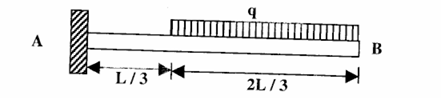
\includegraphics[width=0.5\linewidth]{figs/Q.30.png}
    \caption{Enter Caption}
    \label{fig:figs/Q.30.png}
\end{figure}
\hfill{GATE 2011 PI}
\begin{enumerate}
\begin{multicols}{2}
    \item $\dfrac{7qL^3}{48EI}$
    \item $\dfrac{13qL^3}{72EI}$
    \item $\dfrac{11qL^3}{60EI}$
    \item $\dfrac{qL^3}{24EI}$
\end{multicols}
\end{enumerate}
\item
A short column of length $L$ having cross-sectional area of $50~\text{mm} \times 100~\text{mm}$ is pinned at the ends. The proportional limit of the column is $250~\text{MPa}$ and modulus of elasticity is $200~\text{GPa}$. The minimum length of the column (in m) at which it will buckle elastically is
\hfill{GATE 2011 PI}
\begin{enumerate}
\begin{multicols}{2}
    \item 5.25
    \item 2.25
    \item 1.65
    \item 1.15
\end{multicols}
\end{enumerate}

\item
In a steady state and adiabatic flow of air through a horizontal nozzle, the pressure and temperature drop from $105~\text{kPa}$ and $300~\text{K}$ to $100~\text{kPa}$ and $296~\text{K}$ respectively. Air is considered to be a perfect gas. Take specific heat at constant pressure $C_p = 1005~\text{J/(kg K)}$, density $\rho = 1.15~\text{kg/m}^3$ and ratio of specific heats $\gamma = 1.4$ for air. If the inlet kinetic energy is negligible, then the velocity of air (in m/s) at the nozzle exit is
\hfill{GATE 2011 PI}
\begin{enumerate}
\begin{multicols}{2}
    \item 85
    \item 90
    \item 93
    \item 96
\end{multicols}
\end{enumerate}

\item
Water is flowing through a horizontal pipe of constant diameter and the flow is laminar. If the diameter of the pipe is increased by 50\% keeping the volume flow rate constant, then the pressure drop in the pipe due to friction will decrease by
\hfill{GATE 2011 PI}
\begin{enumerate}
\begin{multicols}{2}
    \item 33\%
    \item 56\%
    \item 70\%
    \item 80\%
\end{multicols}
\end{enumerate}

\item
Cold water flowing at $0.1~\text{kg/s}$ is heated from $20^\circ$C to $70^\circ$C in a counter-flow type heat exchanger by a hot water stream flowing at $0.1~\text{kg/s}$ and entering at $90^\circ$C. The specific heat of water is $4200~\text{J/(kg K)}$ and density is $1000~\text{kg/m}^3$. If the overall heat transfer coefficient $U$ for the heat exchanger is $2000~\text{W/(m}^2~\text{K)}$, the required heat exchange area (in m$^2$) is

\hfill{GATE 2011 PI}
\begin{enumerate}
\begin{multicols}{2}
    \item 0.052
    \item 0.525
    \item 0.151
    \item 0.202
\end{multicols}
\end{enumerate}
\item
Match the following materials with their most appropriate application: 

\begin{tabbing}
    \hspace{6cm} \= \hspace{4cm} \= \kill
    \textbf{Material} \> \textbf{Application} \\[6pt]
    1. Low carbon steel \> P. Machine tool base \\
    2. Stainless steel \> Q. Aircraft parts \\
    3. Gray cast iron \> R. Kitchen utensils \\
    4. Titanium alloys \> S. Car body panels \\
\end{tabbing}
\hfill{GATE 2011 PI}
\begin{enumerate}
\begin{multicols}{2}
    \item 1-P, 2-R, 3-Q, 4-S
    \item 1-P, 2-R, 3-S, 4-Q
    \item 1-S, 2-Q, 3-P, 4-R
    \item 1-S, 2-R, 3-P, 4-Q
\end{multicols}
\end{enumerate}

\item
In a sand casting process, a sphere and a cylinder of equal volumes are separately cast from the same molten metal under identical conditions. The height and diameter of the cylinder are equal. The ratio of the solidification time of the sphere to that of the cylinder is
\hfill{GATE 2011 PI}
\begin{enumerate}
\begin{multicols}{2}
    \item 1.14
    \item 0.87
    \item 1.31
    \item 0.76
\end{multicols}
\end{enumerate}

\item
The thickness of a plate is reduced from $30\, \mathrm{mm}$ to $10\, \mathrm{mm}$ by successive cold rolling passes using identical rolls of diameter $600\, \mathrm{mm}$. Assume that there is no change in width. If the coefficient of friction between the rolls and the work piece is 0.1, the minimum number of passes required is
\hfill{GATE 2011 PI}
\begin{enumerate}
\begin{multicols}{2}
    \item 3
    \item 4
    \item 6
    \item 7
\end{multicols}
\end{enumerate}

\item
Match the following:

\begin{tabbing}
    \hspace{6cm} \= \hspace{4cm} \= \kill
    \textbf{Type of material} \> \textbf{Name of material} \\[6pt]
    1. Thermoplastics \> P. SiAlON \\
    2. Thermosets \> Q. Polyvinylchloride \\
    3. Elastomers \> R. Epoxy \\
    4. Ceramics \> S. Latex \\
\end{tabbing}
\hfill{GATE 2011 PI}
\begin{enumerate}
\begin{multicols}{2}
    \item 1-Q, 2-R, 3-S, 4-P
    \item 1-R, 2-Q, 3-S, 4-P
    \item 1-S, 2-R, 3-Q, 4-P
    \item 1-R, 2-Q, 3-P, 4-S
\end{multicols}
\end{enumerate}
\item
While removing material from iron (atomic weight = 56, valency = 2 and density = $7.8~\text{g/cc}$) by electrochemical machining, a metal removal rate of 2 cc/min is desired. The current (in A) required for achieving this material removal rate is
\hfill{GATE 2011 PI}
\begin{enumerate}
\begin{multicols}{2}
    \item 896.07
    \item 14.93
    \item 448.03
    \item 53764.29
\end{multicols}
\end{enumerate}

\item
To measure the effective diameter of an external metric thread (included angle is $60^\circ$) of 3.5 mm pitch, a cylindrical standard of 30.5 mm diameter and two wires of 2 mm diameter each are used. The micrometer readings over the standard and over the wires are 16.532 mm and 15.398 mm, respectively. The effective diameter (in mm) of the thread is
\hfill{GATE 2011 PI}
\begin{enumerate}
\begin{multicols}{2}
    \item 33.366
    \item 30.397
    \item 29.366
    \item 26.397
\end{multicols}
\end{enumerate}

\item
Observation of a slip gauge on a flatness interferometer produced fringe counts numbering 10 and 14 for two readings. The second reading is taken by rotating the set-up by $180^\circ$. Assume that both faces of the slip gauge are flat and the wavelength of the radiation is $0.5086~\mu$m. The parallelism error (in $\mu$m) between the two faces of the slip gauge is
\hfill{GATE 2011 PI}
\begin{enumerate}
\begin{multicols}{2}
    \item 0.2543
    \item 1.172
    \item 0.5086
    \item 0.1272
\end{multicols}
\end{enumerate}

\item
A shop-floor engineer is looking at an $\overline{X}$ control chart for outer diameter of a cylindrical component with design specifications as $50 \pm 0.1~\text{mm}$. The control chart uses a sample size of 25, and has a standard deviation of 0.01 mm and a mean of 50.02 mm. The process capability index $C_p$ for this process is
\hfill{GATE 2011 PI}
\begin{enumerate}
\begin{multicols}{2}
    \item 0.667
    \item 0.752
    \item 0.565
    \item 0.800
\end{multicols}
\end{enumerate}
\item
The output '$y$' of a process is related to two independent and non-correlated process variables $x_1$ and $x_2$ through the following relation:
\[
y = 200 + 3x_1 - 8x_2
\]
The standard deviations of the variables $x_1$ and $x_2$ are 0.5 each. A portion of cumulative standard normal distribution table (z table) is given below:

\[
\begin{array}{c|ccccc}
z & 1.0 & 1.5 & 2.0 & 2.5 \\
\hline
\text{Cumulative probability} & 0.8413 & 0.9332 & 0.9772 & 0.9938 \\
\end{array}
\]

If the values of $x_1$ and $x_2$ are set at 10 and 20 respectively, the probability that the value of '$y$' is greater than 76.41 will be
\hfill{GATE 2011 PI}
\begin{enumerate}
\begin{multicols}{2}
    \item 0.1587
    \item 0.0062
    \item 0.0228
    \item 0.0668
\end{multicols}
\end{enumerate}

\item The average demand for a component is 10 units per day. A store follows a periodic review system for this component. The stock level for this component is checked after every 30 days. The lead time to get this component from the supplier is 5 days. During one review, the stock level is found to be 50. If the policy of the company is to have a safety stock of 20\% of the expected demand during the next period, order size for the next period will be

\hfill{GATE 2011 PI}
\begin{enumerate}
\begin{multicols}{2}
    \item 340
    \item 350
    \item 360
    \item 370
\end{multicols}
\end{enumerate}

\item A company proposes to spend Rs 2,00,000 for a new machine. The service life of the machine is three years and the minimum acceptable rate of return per year is 25\%. The annual savings (in rupees) due to the machine, assumed to incur at the year end, should be at least

\hfill{GATE 2011 PI}
\begin{enumerate}
\begin{multicols}{2}
    \item 1,30,950
    \item 1,18,340
    \item 1,02,460
    \item 86,500
\end{multicols}
\end{enumerate}

\item An operation consists of four work elements with the following data obtained during a work measurement exercise:

\begin{tabular}{|c|c|c|}
    \hline
    Element No. & Average element time & Rating factor \\
                & (in centi-minutes)  &              \\
    \hline
    1 & 40 & 1.00 \\
    2 & 50 & 1.05 \\
    3 & 45 & 1.10 \\
    4 & 40 & 0.90 \\
    \hline
\end{tabular}

If the total permissible allowance is 11\% of the standard time, then the standard time (in minutes) for the operation would be

\hfill{GATE 2011 PI}
\begin{enumerate}
\begin{multicols}{2}
    \item 2.2
    \item 2.0
    \item 1.8
    \item 1.6
\end{multicols}
\end{enumerate}
\item A small project is composed of seven activities whose time estimates are given below. The activities are identified by their beginning nodes ($i$) and ending nodes ($j$).

\begin{tabular}{|c|c|c|c|c|}
    \hline
    (i) & (j) & \textbf{Optimistic time} (days) & \textbf{Pessimistic time} (days) & \textbf{Most likely time} (days) \\
    \hline
    1 & 2 & 2 & 8 & 2 \\
    1 & 3 & 2 & 8 & 5 \\
    1 & 4 & 3 & 9 & 3 \\
    2 & 5 & 2 & 2 & 2 \\
    3 & 5 & 3 & 15 & 6 \\
    4 & 6 & 3 & 9 & 6 \\
    5 & 6 & 4 & 16 & 7 \\
    \hline
\end{tabular}

The expected project completion time (in days) is
\hfill{GATE 2011 PI}
\begin{enumerate}
\begin{multicols}{2}
    \item 20
    \item 25
    \item 30
    \item 40
\end{multicols}
\end{enumerate}
Common Data Questions
Common Data for Questions 48 and 49:

In a multi-pass drawing operation, a round bar of 10 mm diameter and 100 mm length is reduced in cross-section by drawing it successively through a series of seven dies of decreasing exit diameter. During each of these drawing operations, the reduction in cross-sectional area is 35\%. The yield strength of the material is 200 MPa. Ignore strain hardening.

\item The total true strain applied and the final length (in mm), respectively, are
\hfill{GATE 2011 PI}
\begin{enumerate}
\begin{multicols}{2}
    \item 2.45 and 817
    \item 2.45 and 345
    \item 3.02 and 2043
    \item 3.02 and 3330
\end{multicols}
\end{enumerate}

\item Neglecting friction and redundant work, the force (in kN) required for drawing the bar through the first die, is
\hfill{GATE 2011 PI}
\begin{enumerate}
\begin{multicols}{2}
    \item 15.71
    \item 10.21
    \item 6.77
    \item 4.39
\end{multicols}
\end{enumerate}

Common Data for Questions 50 and 51:

In an acceptance sampling plan, one item is taken at random from the lot and inspected. If the item is good, the lot is accepted, otherwise it is rejected. If the lot is rejected, it is subjected to 100\% inspection and all defective items in the lot are identified and replaced with good items.

\item The slope of the operating characteristic curve (OC Curve) of this plan would be
\hfill{GATE 2011 PI}
\begin{enumerate}
\begin{multicols}{2}
    \item zero
    \item +1
    \item --1
    \item --2
\end{multicols}
\end{enumerate}

\item If the lot size is 50 and it has 10\% defective items, then the average total number of items inspected (ATI) per lot would be
\hfill{GATE 2011 PI}
\begin{enumerate}
\begin{multicols}{2}
    \item 5.9
    \item 7.2
    \item 9.3
    \item 11.5
\end{multicols}
\end{enumerate}
Statement for Linked Answer Questions 52 and 53:

During orthogonal machining of a mild steel specimen with a cutting tool of zero rake angle, the following data is obtained:\\
Uncut chip thickness = 0.25 mm\\
Chip thickness = 0.75 mm\\
Width of cut = 2.5 mm\\
Normal force = 950 N\\
Thrust force = 475 N

\item The shear angle and shear force, respectively, are
\hfill{GATE 2011 PI}
\begin{enumerate}
\begin{multicols}{2}
    \item $71.565^\circ$, 150.21 N
    \item $9.218^\circ$, 861.64 N
    \item $18.435^\circ$, 751.04 N
    \item $23.157^\circ$, 686.66 N
\end{multicols}
\end{enumerate}

\item The ultimate shear stress (in N/mm$^2$) of the work material is
\hfill{GATE 2011 PI}
\begin{enumerate}
\begin{multicols}{2}
    \item 235
    \item 139
    \item 564
    \item 380
\end{multicols}
\end{enumerate}

Statement for Linked Answer Questions 54 and 55:

A system contains four components A, B, C and D. Their time-to-failure distributions are exponential. The mean time to failure (in hours) is found to be 5000, 4000, 4000 and 5000 for A, B, C and D, respectively.

\item The reliabilities $R_A$, $R_B$, $R_C$ and $R_D$ for these four components after 1000 hours of operation will be
\hfill{GATE 2011 PI}
\begin{enumerate}
\begin{multicols}{2}
    \item $R_A = 0.855$, $R_B = 0.8$, $R_C = 0.8$ and $R_D = 0.855$
    \item $R_A = 0.753$, $R_B = 0.9$, $R_C = 0.9$ and $R_D = 0.753$
    \item $R_A = 0.951$, $R_B = 0.852$, $R_C = 0.852$ and $R_D = 0.951$
    \item $R_A = 0.819$, $R_B = 0.779$, $R_C = 0.779$ and $R_D = 0.819$
\end{multicols}
\end{enumerate}
\item 
If the four components in the previous question are connected in a series -parallel structure as shown in the fig , the system reliability at the end of 1000 hours of operation will be
\begin{figure}[H]
    \centering
    
\includegraphics[width=0.5\linewidth]{figs/Q.55.png}
    \caption{fig4}
    \label{fig:figs/Q.55.png}
\end{figure}
\hfill{GATE 2011 PI}
\begin{enumerate}
\begin {multicols}{4}

    \item 0.853
    \item 0.638
    \item 0.733
    \item 0.925
    \end{multicols}
\end{enumerate}
General Aptitude (GA) Questions\\
56-60 carry one mark each
\item Choose the word from the options given below that is most nearly opposite in meaning to the given word: \\
Amalgamate
\hfill{GATE 2011 PI}
\begin{enumerate}
\begin{multicols}{2}
    \item merge
    \item split
    \item collect
    \item separate
\end{multicols}
\end{enumerate}

\item If $\log(P) = (1/2)\log(Q) = (1/3)\log(R)$, then which of the following options is \textit{TRUE}?

\hfill{GATE 2011 PI}
\begin{enumerate}
\begin{multicols}{2}
    \item $P^2 = Q^3 R^2$
    \item $Q^2 = PR$
    \item $Q^2 = R^3 P$
    \item $R = P^2 Q^2$
\end{multicols}
\end{enumerate}

\item Choose the most appropriate word from the options given below to complete the following sentence.\\
If you are trying to make a strong impression on your audience, you cannot do so by being understated, tentative or \underline{\hspace{2.2cm}}.
\hfill{GATE 2011 PI}
\begin{enumerate}
\begin{multicols}{2}
    \item hyperbolic
    \item restrained
    \item argumentative
    \item indifferent
\end{multicols}
\end{enumerate}

\item Which of the following options is the closest in meaning to the word below: \\
Inexplicable
\hfill{GATE 2011 PI}
\begin{enumerate}
\begin{multicols}{2}
    \item Incomprehensible
    \item Indelible
    \item Inextricable
    \item Infallible
\end{multicols}
\end{enumerate}

\item Choose the most appropriate word(s) from the options given below to complete the following sentence.\\
I contemplated \underline{\hspace{1.5cm}} Singapore for my vacation but decided against it.
\hfill{GATE 2011 PI}
\begin{enumerate}
\begin{multicols}{2}
    \item to visit
    \item having to visit
    \item visiting
    \item for a visit
\end{multicols}
\end{enumerate}
61 to 65 carry two marks each
\item A container originally contains 10 litres of pure spirit. From this container 1 litre of spirit is replaced with 1 litre of water. Subsequently, 1 litre of the mixture is again replaced with 1 litre of water and this process is repeated one more time. How much spirit is now left in the container?
\hfill{GATE 2011 PI}
\begin{enumerate}
\begin{multicols}{4}
    \item 7.58 litres
    \item 7.84 litres
    \item 7 litres
    \item 7.29 litres
\end{multicols}
\end{enumerate}
\item 
P, Q, R and S are four types of dangerous microbes recently found in a human habitat. The area of each circle with its diameter printed in brackets represents the growth of a single microbe surviving human immunity system within 24 hours of entering the body. The danger to human beings varies proportionately with the toxicity, potency and growth attributed to a microbe shown in the figure below:
\begin{figure}[H]
    \centering
    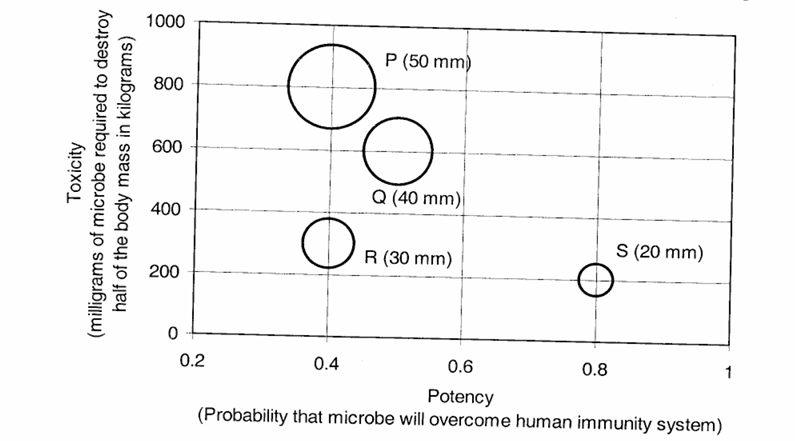
\includegraphics[width=0.5\linewidth]{figs/Q.62.png}
    \caption{fig5}
    \label{fig:figs/Q.62.png}
\end{figure}
a pharmaceutical company is contemplating the devolopment of a vaccine against the most dangerous microbe.Which microbe should the company target first attempt?

\hfill{GATE 2011 PI}
\begin{enumerate}
\begin{multicols}{4}
    \item P
    \item Q
    \item R
    \item S
\end{multicols}
\end{enumerate}
\item A transporter receives the same number of orders each day. Currently, he has some pending orders (backlog) to be shipped. If he uses 7 trucks, then at the end of the 4th day he can clear all the orders. Alternatively, if he uses only 3 trucks, then all the orders are cleared at the end of the 10th day. What is the minimum number of trucks required so that there will be no pending order at the end of the 5th day?
\hfill{GATE 2011 PI}
\begin{enumerate}
\begin{multicols}{2}
    \item 4
    \item 5
    \item 6
    \item 7
\end{multicols}
\end{enumerate}

\item Few school curricula include a unit on how to deal with bereavement and grief, and yet all students at some point in their lives suffer from losses through death and parting.

Based on the above passage which topic would not be included in a unit on bereavement?

\hfill{GATE 2011 PI}
\begin{enumerate}
\begin{multicols}{2}
    \item how to write a letter of condolence
    \item what emotional stages are passed through in the healing process
    \item what the leading causes of death are
    \item how to give support to a grieving friend
\end{multicols}
\end{enumerate}

\item The variable cost (V) of manufacturing a product varies according to the equation $V = 4q$, where $q$ is the quantity produced. The fixed cost (F) of production of same product reduces with $q$ according to the equation $F = 100/q$. How many units should be produced to minimize the total cost $(V+F)$?
\hfill{GATE 2011 PI}
\begin{enumerate}
\begin{multicols}{4}
    \item 5
    \item 4
    \item 7
    \item 6
\end{multicols}
\end{enumerate}

















    







































    





















































\end{enumerate}


\end{document}
